% no notes
\documentclass[dvipsnames]{beamer}
% notes and slides
%\documentclass[notes]{beamer}
% notes only
% \documentclass[notes=only]{beamer}
\usepackage{graphicx} % Allows including images
\usepackage{booktabs} % Allows the use of \toprule, \midrule and \bottomrule in tables
\usepackage{multirow}
\usepackage{multimedia}
\usepackage{tikz}
\usepackage{circuitikz}
\usepackage{url}
\usepackage{pgfplots}
\pgfplotsset{compat=newest}
\usepgfplotslibrary{groupplots,dateplot}
\usetikzlibrary{patterns,shapes.arrows}
\usepackage{standalone}
\usepackage{adjustbox}
\usepackage{lmodern}
\usepackage{pgfplots}
\usepackage{amsmath}
\usepackage{amsthm}
\usepackage{multimedia}
\usepackage{standalone}
\usepackage{csquotes}
\usepackage{caption}
\usepackage{subcaption}


\DeclareMathOperator*{\argmax}{argmax}
\DeclareMathOperator*{\argmin}{argmin}
\def\ie{i.e.\ }
\def\eg{e.g.\ }
\newcommand{\twovartext}[3]{\underbrace{#1}_{\substack{\text{#2} \\ \text{#3}}}}
\newcommand{\vartext}[2]{\underbrace{#1}_{\text{#2}}}

\newcommand{\referencefootnote}[1]{\setbeamertemplate{footline}[text line]{%%%
\parbox{0.9\paperwidth}{\vspace*{-23pt}\tiny{\textcolor{gray}{#1}}\hfill\scriptsize\insertframenumber}}}

% Redefine the caption format to remove "Figure"
\captionsetup[figure]{labelformat=empty}
  

\PassOptionsToPackage{american}{babel} % change this to your language(s), main language last
% Spanish languages need extra options in order to work with this template
% \PassOptionsToPackage{spanish,es-lcroman}{babel}
\usepackage{babel}

\PassOptionsToPackage{%
  backend=biber,bibencoding=utf8, %instead of bibtex
  %backend=bibtex8,bibencoding=ascii,%
  language=auto,%
  style=numeric-comp,%
  %style=authoryear-comp, % Author 1999, 2010
  %bibstyle=authoryear,dashed=false, % dashed: substitute rep. author with ---
  style=alphabetic,
  sorting=nyt, % name, year, title
  maxbibnames=10, % default: 3, et al.
  %backref=true,%
  %natbib=true % natbib compatibility mode (\citep and \citet still work)
}{biblatex}
\usepackage{biblatex}

\addbibresource{bib.bib}

\usetheme{metropolis}           % Use metropolis theme
\setbeamertemplate{caption}[default]
\title{Machine Learning Basics}
\date{November 30, 2023}%{\today}
\institute{Visual Computing Group, Uni Bonn}
\author{Elena Trunz}

\titlegraphic{\includegraphics[width=2.00cm]{UNI_Bonn_Logo_Standard_RZ.pdf}}
\begin{document}
    \maketitle

    \begin{frame}
    \frametitle{Overview} 
    \tableofcontents
    \end{frame}

   	\let\oldfootnoterule\footnoterule
	\def\footnoterule{\only<3->\oldfootnoterule}
    \section{Machine Learning Algorithms}
    \begin{frame}{What is machine learning?}
			Machine learning is a subfield of artificial intelligence with the goal of developing algorithms capable of learning
from data automatically. \pause

			What do we mean by learning? \pause

			"A computer program is said to learn from \emph{experience} $E$ with respect to some
class of \emph{tasks} $T$ and \emph{performance measure} $P$, if its performance at tasks in $T$, as
measured by $P$, improves with experience $E$." (Mitchell, 1997\footnote<3->{ Mitchell, T. M. (1997). Machine Learning. McGraw-Hill, New York.})

    \end{frame}
		
		\begin{frame}{Experience $E$}
		The experience $E$ is the information that the algorithm can use during learning:
		\begin{itemize}
			\item \emph{dataset} 
			\item aka (training) data
		\end{itemize} \pause

		Dataset contains \emph{examples} (\emph{data points}): collection of \emph{features} that have been quantitatively measured from some object or event
		\begin{itemize}
			\item $m$-dimensional data point: $\mathbf{x} \in \mathbb{R}^m$
			\item each entry $x_i$ is another feature
		\end{itemize}
    \end{frame}
		\note{Beispiele: images (features are values of the pixels in the image), patient data (features are age, height, weight etc), weather data etc}
		
				
		{ \referencefootnote{Alex Krizhevsky "Learning Multiple Layers of Features from Tiny Images", 2009.}
	\begin{frame}{Example dataset: CIFAR10 }
		%\begin{itemize}
			%\item 10 classes
			%\item 50,000 training images 
			%\item 10,000 testing images
		%\end{itemize}
		%\begin{figure}
			%\includegraphics[scale=.2]{figures/cifar2.png}
			%\end{figure}
			\begin{figure}[htbp]
					\begin{minipage}[t]{6cm}
						\vspace{0pt}
						%\centering
						\includegraphics[scale=.23]{figures/cifar2.png}
						%\caption{Bild1}
						%\label{fig:Bild1}
					\end{minipage}
					\hspace{0.8cm} %\hfill
					\begin{minipage}[t]{3.7cm}
						\vspace{50pt}
								\scriptsize
								\begin{itemize}
									\item[] 10 classes
									\item[] 50,000 training images 
									\item[] 10,000 testing images
								\end{itemize}
					\end{minipage}
				\end{figure}
    \end{frame}
		}
		
	%\let\oldfootnoterule\footnoterule
	\def\footnoterule{\only<1->\oldfootnoterule}
	\begin{frame}{Example dataset: Iris}
		Iris dataset\footnote{\url{https://archive.ics.uci.edu/ml/datasets/iris}} \pause
		\begin{itemize}
			\item Collection of measurements of different parts of 150 iris plants\pause
			\item Each individual plant coresponds to one example \pause
			\item The features within each example are\pause
			\begin{itemize}
				\item sepal length
				\item sepal width
				\item petal length
				\item petal width \pause
			\end{itemize}
			\item Recording, which species each plant belonged to \pause
			\item Three different species of iris plants
		\end{itemize}
    \end{frame}
		
		\begin{frame}{Supervised vs. unsupervised learning}
			\emph{Supervised} learning:
			\begin{itemize}
				\item Each data point $\mathbf{x}$ comes with an associated \emph{label} or \emph{target} value $\mathbf{y}$
				\item The algorithm is learned by trying to match the targets, or predict $\mathbf{y}$ from $\mathbf{x}$
				\item From a probabilistic sense this corresponds to estimating $P(\mathbf{y} | \mathbf{x})$
			\end{itemize}
			\pause

			\emph{Unsupervised} learning:
			\begin{itemize}
				\item Only data points $\mathbf{x}$, no \emph{labels}
				\item The goal is to uncover the inherent structure within the data
				\item From a probabilistic sense this corresponds to estimating \emph{data generating distribution} $p_{\text{data}}(\mathbf{x})$
			\end{itemize}
			\note{Beispiele mit Iris dataset: Supervised: Classifikation: bestimme eine der drei klassen, anhand von features. Unsupervised: bestimme data generating distribution for synthesis of new iris examples}
    \end{frame}
		
		\begin{frame}{Machine learning tasks}
Tasks specify how a machine learning system should process \emph{examples}. Common tasks include \pause


\begin{itemize}
\item \textbf{classification}: determine category of input \ie $f: \mathbb{R}^m \rightarrow \{1, ..., K\}$ \pause

\item \textbf{regression}: predict numerical value(s) for some input, \ie  $f: \mathbb{R}^m \rightarrow \mathbb{R}^p$ \pause

\item \textbf{density estimation}: learn probability density (if $\mathbf{x}$ is continuous) or probability mass (if $\mathbf{x}$ is discrete) function $p_{\text{model}}: \mathbb{R}^m \rightarrow \mathbb{R}$ on the space that the examples were drawn from \pause

\item \textbf{dimensionality reduction}:  find a compact, lower-dimensional representation of high-dimensional data $\mathbf{x} \in \mathbb{R}^D$, which is often easier to analyze than the original data
\end{itemize}

\end{frame}

		\begin{frame}{More machine learning tasks}
\begin{itemize}
\item \textbf{imputation of missing values} or \textbf{hole filling}: predict values of missing entries $x_i$ of $\mathbf{x} \in \mathbb{R}^m$ \pause

\item \textbf{structured prediction}: vector output with well-defined relationships between the elements \pause

\item \textbf{synthesis}: generation of new examples that are similar to the training data \pause

\item \textbf{denoising}: get \emph{clean} example $\mathbf{x} \in \mathbb{R}^m$ from \emph{corrupted} example $\tilde{\mathbf{x}} \in \mathbb{R}^m$ %, i.e. prediction of $p(\mathbf{x} | \tilde{\mathbf{x}})$ 
%\item \textbf{hole filling}: inpainting for an example $\mathbf{x} \in \mathbb{R}^m$ with missing entries $x_i$
\end{itemize}
\note{hole filling aka inpainting}
\end{frame}
		
		\begin{frame}{Performance measure $P$}
			To evaluate a machine learning algorithm, we must design a quantitative measure of its performance.
			
			Performance measure is task-spesific:
			\begin{itemize}
				\item Classification and imputation of missing inputs: 
				\begin{itemize}
					\item \emph{Accuracy}: proportion of examples for which the model produces the correct output
					\item \emph{Error rate}: proportion of examples for which the model produces an incorrect output
				\end{itemize}  
				\item Density estimation: 
					\begin{itemize}
						\item Average log-probability the model assigns to examples
					\end{itemize}  
			\end{itemize}

    \end{frame}
		\note{
The choice of performance measure may seem straightforward and objective, but it is often difficult to choose a performance measure that corresponds well to the desired behaviour of the system.
In some cases, this is because it is difficult to decide what should be measured. For example, when performing a transcription task, should we measure the accuracy of the system at transcribing entire sequences, or should we use a more fine-grained performance measure that gives partial credit for getting some elements of the sequence correct? When performing a regression task, should we penalize the system more if it frequently makes medium-sized mistakes or if it rarely makes very large mistakes? These kinds of design choices depend on the application.
In other cases, we know what quantity we would ideally like to measure, but measuring it is impractical. For example, this arises frequently in the context of density estimation. Many of the best probabilistic models represent probability distributions only implicitly. Computing the actual probability value assigned to a specific point in space in many such models is intractable. In these cases, one must design an alternative criterion that still corresponds to the design objectives, or design a good approximation to the desired criterion.
}
		
		\begin{frame}{Generalization}
		We want to evaluate performance of our system on data that it has \emph{not yet seen}. \pause
		
		This estimates how well the system will \emph{generalize}, in comparison to performance on already seen data used during the learning process. 
		\pause
		\begin{itemize}
			\item Unseen data makes up our \emph{test set} or test data \pause
			\item Already seen data is the \emph{training set} or training data \pause
		\end{itemize}

	  During training we want to reduce the \emph{training error} -- this is simply an optimization problem.  \pause 
		
		What distinguishes learning from optimization is the interest in also reducing the \emph{test error} (\emph{generalization error}).
		\end{frame}
		
				\begin{frame}{Loss function}
			A \emph{loss function} is a function that measures the difference (or loss) between a predicted label and a true label \pause
			
			It is closely related to performance measure: \pause
			\begin{itemize}
				\item Loss function is used \emph{during} the training to \emph{train} the model \pause
				\item Performance measure is used \emph{after} the training to \emph{evaluate} the model \pause
			\end{itemize}
			
			Sometimes both can be represented by the same function (as it is in the case of regression), but for some other tasks (\eg classification) we have different measures (\eg cross-entropy vs. accuracy).
		\end{frame}
		
			\section{Image Classification}
    \begin{frame}{Classification task}
			\emph{Given:} 
			\begin{itemize}
				\item Input examples
				\item Corresponding labels
			\end{itemize}
			
			\emph{Find:} Classifier that predicts a class from the input.
			
			Example: given an x-ray image, predict if the person is sick.
    \end{frame}
{ \referencefootnote{\href{https://www.flickr.com/photos/tjukka2/8565139583/sizes/l/}{\underline{This image}} by \href{https://www.flickr.com/photos/tjukka2/}{\underline{Tjukka2}} is licensed under \href{https://creativecommons.org/licenses/by-nc-sa/2.0/}{CC-BY-SA 2.0}.}
\begin{frame}{Image classification}
				\begin{figure}[htbp]
					\begin{minipage}[t]{5.5cm}
						\vspace{0pt}
						%\centering
						\includegraphics[scale=.4]{figures/cat4.jpg}
						%\caption{Bild1}
						%\label{fig:Bild1}
					\end{minipage}
					\hspace{1.5cm} %\hfill
					\begin{minipage}[t]{2.5cm}
						\vspace{50pt}
						$\longrightarrow$ \quad cat
					\end{minipage}
				\end{figure}
\end{frame}
\note{given descrete set of lables, dog, cat, plane, boat etc.}
}
\begin{frame}{Semantic gap}
\begin{figure}
  \begin{subfigure}{0.45\linewidth} 
    \centering
    \includegraphics[width=5cm]{figures/cat4.jpg}
    \caption*{What we see}
    \label{fig:subfig1}
  \end{subfigure}
  \hfill
  \begin{subfigure}{0.45\linewidth}
    \centering
   \includegraphics[width=5cm, height=3.75cm]{figures/test_2.png}
    \caption*{What the computer sees}
    \label{fig:subfig2}
  \end{subfigure}
  %\caption{Main Caption for Both Figures}
	\begin{itemize}
		\item An image is just a grid of numbers between 0 and 255
		\item E.g. this RGB image: $300\times 400 \times 3$
	\end{itemize}
  \label{fig:main}
\end{figure}
\end{frame}
\note{if camera moves, this grid containes a totally different grid}

{ \referencefootnote{\href{https://www.flickr.com/photos/andymiccone/29212712404/}{\underline{This}}, \href{https://www.flickr.com/photos/imoviesh/29065050008/}{\underline{this}}, \href{https://www.flickr.com/photos/imoviesh/40034063605/}{\underline{this}} and \href{https://www.flickr.com/photos/imoviesh/28877326228/}{\underline{this}} images are \href{https://creativecommons.org/publicdomain/zero/1.0/deed.en}{\underline{CC0 1.0}} public domain.}
\begin{frame}{Challenges: deformation}
\begin{figure}
\includegraphics[height =3cm]{figures/def1.jpg}
\includegraphics[height =3cm]{figures/def2.jpg}
\includegraphics[height =3cm]{figures/def3.jpg}
\includegraphics[height =3cm]{figures/def4.jpg}
\end{figure}
\end{frame}
}
{ \referencefootnote{\href{https://www.flickr.com/photos/imoviesh/41228156474/}{\underline{This}}, \href{https://www.flickr.com/photos/langithijau/3803523814/}{\underline{this}} and \href{https://www.flickr.com/photos/imoviesh/39738183494/}{\underline{this}} images are \href{https://creativecommons.org/publicdomain/zero/1.0/deed.en}{\underline{CC0 1.0}} public domain.}
\begin{frame}{Challenges: occlusion}
\begin{figure}
\includegraphics[height =2.5cm]{figures/occ1.jpg}
\includegraphics[height =2.5cm]{figures/occ2.jpg}
\includegraphics[height =2.5cm]{figures/occ3.jpg}
\end{figure}
\end{frame}
}
{ \referencefootnote{\href{https://www.flickr.com/photos/kartlyn/38205483234/in/photostream/}{\underline{This}}, \href{https://www.flickr.com/photos/perdidoenelsiglo/24680737334/}{\underline{this}} and \href{https://www.flickr.com/photos/dcoetzee/3566532901/}{\underline{this}} images are \href{https://creativecommons.org/publicdomain/zero/1.0/deed.en}{\underline{CC0 1.0}} public domain.}
\begin{frame}{Challenges: illumination}
\begin{figure}
\includegraphics[height =2.7cm]{figures/illu1.jpg}
\includegraphics[height =2.7cm]{figures/illu2.jpg}
\includegraphics[height =2.7cm]{figures/illu3.jpg}
\end{figure}
\end{frame}
}
{ \referencefootnote{\href{https://pixabay.com/photos/cat-camouflage-fall-fur-animals-408728/}{\underline{This image}} is \href{https://creativecommons.org/publicdomain/zero/1.0/deed.en}{\underline{CC0 1.0}} public domain.}
\begin{frame}{Challenges: background clutter}
\begin{figure}
\includegraphics[scale=.35]{figures/clutter2.jpg}
\end{figure}
\end{frame}
}
{ \referencefootnote{\href{https://www.flickr.com/photos/142147129@N03/26374109870/in/photostream/}{\underline{This}} and \href{https://www.flickr.com/photos/125779345@N05/23447418723/}{\underline{this}} images are \href{https://creativecommons.org/publicdomain/zero/1.0/deed.en}{\underline{CC0 1.0}} public domain.}
\begin{frame}{Challenges: intraclass variation}
\begin{figure}
\includegraphics[height =5cm]{figures/intra2.jpg} \quad
\includegraphics[height =5cm]{figures/intra1.jpg}
\end{figure}
\end{frame}
}
\begin{frame}{A rule-based image classifier}
\begin{figure}
\includegraphics[scale=.7]{figures/rule_based.png}
\end{figure}
\begin{itemize}
	\item There are many rule-based algorithms for \eg sorting a list of numbers
	\item No obvious way to hard-code the algorithm for recognizing a cat or other classes
\end{itemize}

\end{frame}

\begin{frame}{Attempts have been made}
\begin{figure}
\includegraphics[scale=.6]{figures/canny.png}
\end{figure}
\end{frame}
\note{}

\begin{frame}{Data-driven classification}
\begin{enumerate}
	\item Collect a dataset of images and labels
	\item Use Machine Learning to train a classifier
	\item Evaluate the classifier on new images
\end{enumerate}
\begin{figure}
\includegraphics[scale=.7]{figures/ml_func.png}
\end{figure}
\end{frame}

\section{Nearest Neighbor Classification}
\begin{frame}{First classifier: Nearest Neighbor}
\begin{figure}
\includegraphics[scale=.7]{figures/knn_func.png}
\end{figure}
\end{frame}

{ \referencefootnote{\href{https://padeprueba.fandom.com/es/wiki/Forma_animal}{\underline{This image}} is licensed under \href{https://creativecommons.org/licenses/by-sa/}{CC-BY-SA}.}
\begin{frame}{What is similarity?}
%The quality or state of being similar; likeness; resemblance; as a similarity of features. \pause
%%\vspace*{-0.04cm}
%\hfill \footnotesize \emph{Webster's Dictionary}
\begin{figure}[htbp]
					\begin{minipage}[t]{5.5cm}
						\vspace{0pt}
						%\centering
						\includegraphics[scale=.5]{figures/similarity.png}
						%\caption{Bild1}
						%\label{fig:Bild1}
					\end{minipage}
					\hspace{1cm} %\hfill
					\begin{minipage}[t]{4cm}
						\vspace{30pt}
						\scriptsize 
						\begin{itemize}
							\item The real meaning of similarity is a philosophical question
							\item We will take a more pragmatic approach
						\end{itemize}
					\end{minipage}
				\end{figure}
\textbf{Definition:} Let $U$ be the universe of possible objects. The \emph{distance} (\emph{dissimilarity, metric}) on $U$ is a function $d: U\times U \rightarrow \mathbb{R}$ that satisfies certain conditions (axioms). 
\end{frame}
}
\note{hart to define, but we know it when we see it}
		
\begin{frame}{Intuition behind axioms of a distance function}
\begin{align*}
		&d(a, b) = 0 \Leftrightarrow a = b  &&\text{\emph{Identity of indiscernibles}} \\
		\intertext{\footnotesize{Otherwise there are objects that differ from each other, but we can't distinguish them.}}
		&d(a, b) = d(b, a) &&\text{\emph{Symmetry}}\\
		\intertext{\footnotesize{Otherwise we could claim "Mary looks like Jenny, but Jenny bears no resemblance to Mary."}}
		&d(a, c) \leq d(a, b) + d(b,c) &&\text{\emph{Triangle inequality}}\\
		\intertext{\footnotesize{Otherwise we could claim "Mary looks like Jenny and Sarah, yet Jenny bears no resemblance to Sarah."}}
\end{align*}
\end{frame}

\begin{frame}{L1 (Manhattan) distance}
One common similarity measure is the L1 distance:
 \[
			d_1(a,b) = \sum_{i=1}^m|a_i-b_i|
	\]

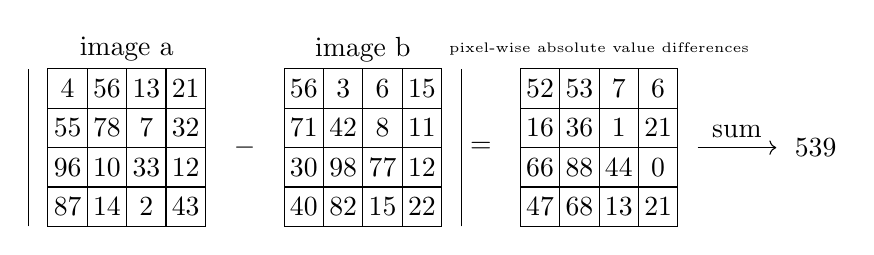
\begin{tikzpicture}[scale=0.5]
  % Draw the left vertical line for the big square
  \draw (0.5,0) -- (0.5,4);
  
  % Draw the first big square (image a)
  \draw (1,0) rectangle (5,4);
  % Add the text "image a" over the first big square
  \node at (3,4.5) {image a};
  
  % Draw the verticalhorizontal lines for subdivision in the first square
  \foreach \x in {2,3,4}
    \draw (\x,0) -- (\x,4);
    
  % Draw the horizontal lines for subdivision in the first square
  \foreach \y in {1,2,3}
    \draw (1,\y) -- (5,\y);

  % Add numbers to the small squares in the first square
  \node at (1.5,3.5) {4};
  \node at (2.5,3.5) {56};
  \node at (3.5,3.5) {13};
  \node at (4.5,3.5) {21};
  
  \node at (1.5,2.5) {55};
  \node at (2.5,2.5) {78};
  \node at (3.5,2.5) {7};
  \node at (4.5,2.5) {32};
  
  \node at (1.5,1.5) {96};
  \node at (2.5,1.5) {10};
  \node at (3.5,1.5) {33};
  \node at (4.5,1.5) {12};
  
  \node at (1.5,0.5) {87};
  \node at (2.5,0.5) {14};
  \node at (3.5,0.5) {2};
  \node at (4.5,0.5) {43};

  % Draw a minus symbol
  \node at (6,2) {$-$};
  
  % Draw the second big square (image b)
  \draw (7,0) rectangle (11,4);
  % Add the text "image b" over the second big square
  \node at (9,4.5) {image b};
  
  % Draw the vertical lines for subdivision in the second square
  \foreach \x in {8,9,10}
    \draw (\x,0) -- (\x,4);
	
	 % Draw the horizontal lines for subdivision in the first square
  \foreach \y in {1,2,3}
    \draw (7,\y) -- (11,\y);
    
  % Add numbers to the small squares in the second square
  \node at (7.5,3.5) {56};
  \node at (8.5,3.5) {3};
  \node at (9.5,3.5) {6};
  \node at (10.5,3.5) {15};
  
  \node at (7.5,2.5) {71};
  \node at (8.5,2.5) {42};
  \node at (9.5,2.5) {8};
  \node at (10.5,2.5) {11};
  
  \node at (7.5,1.5) {30};
  \node at (8.5,1.5) {98};
  \node at (9.5,1.5) {77};
  \node at (10.5,1.5) {12};
  
  \node at (7.5,0.5) {40};
  \node at (8.5,0.5) {82};
  \node at (9.5,0.5) {15};
  \node at (10.5,0.5) {22};

  % Draw the right vertical line for the second square
  \draw (11.5,0) -- (11.5,4);
  
  % Draw the equal sign
  \node at (12,2) {$=$};
  
  % Draw the third big square (image c)
  \draw (13,0) rectangle (17,4);
  % Add the text "image c" over the third big square
  \node at (15,4.5) {\tiny pixel-wise absolute value differences};
  
  % Draw the vertical lines for subdivision in the third square
  \foreach \x in {14,15,16}
    \draw (\x,0) -- (\x,4);
    
  % Draw the horizontal lines for subdivision in the third square
  \foreach \y in {1,2,3}
    \draw (13,\y) -- (17,\y);

  % Add numbers to the small squares in the third square
  \node at (13.5,3.5) {52};
  \node at (14.5,3.5) {53};
  \node at (15.5,3.5) {7};
  \node at (16.5,3.5) {6};
  
  \node at (13.5,2.5) {16};
  \node at (14.5,2.5) {36};
  \node at (15.5,2.5) {1};
  \node at (16.5,2.5) {21};
  
  \node at (13.5,1.5) {66};
  \node at (14.5,1.5) {88};
  \node at (15.5,1.5) {44};
  \node at (16.5,1.5) {0};
  
  \node at (13.5,0.5) {47};
  \node at (14.5,0.5) {68};
  \node at (15.5,0.5) {13};
  \node at (16.5,0.5) {21};
	  % Add the right arrow pointing to the number 456
  \draw[->] (17.5,2) -- (19.5,2) node[midway,above] {sum};
  \node at (20.5,2) {539};
\end{tikzpicture}

%\begin{figure}
%\includegraphics[scale=.4]{figures/L1.png}
%\end{figure}
\end{frame}

\begin{frame}{NN results on CIFAR10}
\begin{figure}
\includegraphics[scale=.45]{figures/1nn_cifar.png}
\end{figure}
\end{frame}

\begin{frame}{Decision regions of NN }
\begin{figure}
\includegraphics[scale=.6]{figures/k_nn_boundary_k1_wotitle.png}
\end{figure}
\end{frame}


\begin{frame}{$k$-Nearest Neighbors classifier}
Instead of copying label from nearest neighbor, take \emph{majority vote} from $k$ closest points: \pause
\begin{figure}
\includegraphics[scale=.33]{figures/k_nn_data.png}
\includegraphics[scale=.33]{figures/k_nn_boundary_k1.png}
\includegraphics[scale=.33]{figures/k_nn_boundary_k5.png}
\includegraphics[scale=.33]{figures/k_nn_boundary_k10.png}
%\caption{Left: $k=1$, middle: $k=3$, right: $k=5$. }
\end{figure}
\end{frame}

\begin{frame}{10-NN results on CIFAR10}
\begin{figure}
\includegraphics[scale=.45]{figures/10nn_cifar.png}
\end{figure}
\end{frame}

	\begin{frame}{L2 (Euclidean) distance}
			Another common similarity measure is the \emph{Euclidean distance}.
			
			The Euclidean distance between two $m$-dimensional points is the length of a line segment between these points
			\[
			d_2(a,b) = \sqrt{\sum_{i=1}^m(a_i-b_i)^2}.
			\]
	\end{frame}
\begin{frame}{Choosing $k$ and distance metric}
What is the best distance?

What is the best value of $k$? \pause

Very problem-dependent! \pause

Try them all out and see what works best
\end{frame}

\section{Linear Regression as ML Algorithm}
		
			\begin{frame}{Linear regression: experience}
			Recall the regression problem: the goal is to build a system that 
			\begin{itemize}
				\item takes a vector $\mathbf{x} \in \mathbb{R}^m$ as input and
				\item predicts the value of a scalar $ y \in \mathbb{R}$ as its output.
			\end{itemize}  \pause
			
			Our experience $E$ are the input examples $\mathbf{X} = \{\mathbf{x}_1,\dots,\mathbf{x}_N\}$ and the corresponding target values $\mathbf{y} \in \mathbb{R}^N$. \pause
			
			Thus, the dataset consists of $N$ example pairs $\{(\mathbf{x}_1,y_1), \dots, (\mathbf{x}_N,y_N)\}$ 
			
			\note{Linear regression refers to models that are linear in the parameters, i.e. models that describe a function by a linear combination of input features.}
		\end{frame}
		
		\begin{frame}{Linear regression: task}
			
			Let $\hat{y}$ be the value that our model predicts $y$ should take on. We define the output to be
			\[
				\hat{y} = \mathbf{w}^{\top}\mathbf{x}
			\]
			where $\mathbf{w}$ is a vector of model \emph{parameters}.
			
			Parameters are values that control the behavior of the system. \pause
			
			$\rightarrow$ Our task $T$: predict $y$ from $\mathbf{x}$ by outputting $\hat{y} = \mathbf{w}^{\top}\mathbf{x}$.
			\note{Parameters are values that control the behavior of the system. In this case, $w_i$ is the coefficient that we multiply by feature $x_i$ before summing up the contributions from all the features. We can think of $w$ as a set of weights that determine how each feature affects the prediction. If a feature $x_i$ receives a positive weight $w_i$, then increasing the value of that feature increases the value of our prediction $\hat{y}$. If a feature receives a negative weight, then increasing the value of that feature decreases the value of our prediction. If a feature’s weight is large in magnitude, then it has a large effect on the prediction. If a feature’s weight is zero, it has no effect on the prediction.}
		\end{frame}
		
		\begin{frame}{Linear regression: performance measure}
			Suppose we have $M$ example inputs together with the correct target values in the test dataset. \pause
			
			One way of measuring the performance of the model for a regression task is to compute the \emph{mean squared error} (MSE):
			\begin{align*}
			MSE_{test} &= \frac{1}{M}\sum_i (\hat{\mathbf{y}}^{(test)} - \mathbf{y}^{(test)})_{i}^2 \\ 
			&= \frac{1}{M}\|\hat{\mathbf{y}}^{(test)} - \mathbf{y}^{(test)}\|_{2}^{2} 
			\end{align*}

		\end{frame}
		
				\begin{frame}{Linear regression: ML algorithm}
				To make a machine learning algorithm, we need to design an algorithm that will improve the parameters $\mathbf{w}$ in a way that reduces $MSE_{test}$ when the algorithm is allowed to gain experience by observing the training set $(\mathbf{X}^{(train)}, \mathbf{y}^{(train)})$. \pause
				
				One way to do it is to minimize $MSE_{train}$. We can simply solve for where the gradient of $MSE_{train}$ is $\mathbf{0}$: \pause
				\[
				\nabla_{\mathbf{w}}MSE_{train} = \mathbf{0} \pause
				\]
				\[
				\nabla_{\mathbf{w}}\frac{1}{M}\|\hat{\mathbf{y}}^{(train)} - \mathbf{y}^{(train)}\|_{2}^{2}  = \mathbf{0} \pause
				\]
				\[
				\frac{1}{M}\nabla_{\mathbf{w}}\|\mathbf{X}^{(train)}\mathbf{w} - \mathbf{y}^{(train)}\|_{2}^{2}  = \mathbf{0} \pause
				\]
				\[
				\Rightarrow \mathbf{w}= (\mathbf{X}^{(train)\top}\mathbf{X}^{(train)})^{-1}\mathbf{X}^{(train)\top}\mathbf{y}^{(train)}
				\]
				
		\end{frame}
		
		{ \referencefootnote{Image was taken from \cite{Goodfellow_et_al_2016}}
			\begin{frame}{Linear regression: result}
				 \begin{figure}
					\center
					\includegraphics[scale=.6]{figures/regression.png} 
					\caption{Training sets consists of ten examples, each containing one feature. So there is only one parameter to learn, $w_1$ (= slope).}
					\end{figure}
		\end{frame}
		}
		\begin{frame}{Linear regression: notes}
		Usually linear regression refers to a model with an additional parameter -- an intercept term $b$:
		\[
		\hat{y} = \mathbf{w}^{\top}\mathbf{x}+b
		\]
		
		This means that the plot of the model's predictions need not pass though the origin.
		
		We can continue to use the model $\hat{y} = \mathbf{w}^{\top}\mathbf{x}$, by implicitly including $b$:
		\begin{itemize}
			\item Augment $\mathbf{x}$ with an extra entry that is always set to 1
			\item The weight corresponding to the extra 1 entry plays the role of the bias parameter $b$
		\end{itemize}
		\end{frame}
		
	\section{Generalization}
	\begin{frame}{Underfitting and overfitting}

How well a machine learning algorithm will perform, depends on its ability to \pause
\begin{enumerate}
\item Make the training error small \pause
\item Make the gap between training and test error small \pause
\end{enumerate}

Algorithms which \emph{underfit}, cannot satisfy the first criteria. \pause

Algorithms which \emph{overfit}, can satisfy the first criteria but not the second.
\end{frame}

\begin{frame}{Model Capacity}
Underfitting and overfitting can be controlled by adjusting the \emph{model capacity} in the learning algorithm.  \pause

A model's capacity is its ability to fit a wide variety of functions. \pause

Models with (too) low capacity are not rich or expressive enough to capture the training data and hence underfit.  \pause

Models with (too) high capacity simply memorize the training data and will therefore overfit. 
\end{frame}
{ \referencefootnote{Image was taken from \cite{Goodfellow_et_al_2016}}
\begin{frame}{Model Capacity (2)}
\begin{itemize}
	\item Capacity can be controlled by the choice of the \emph{hypothesis space}. This space determines the set of functions that the learning algorithm can select as being the solution.  \pause
	\item The linear regression algorithm has the set of all linear functions of its input as its hypothesis space. \pause
	\item We can increase the model's capacity by generalizing linear regression to include polynomials in its hypothesis space. 
\end{itemize}
 \begin{figure}
		\center
		\includegraphics[scale=.35]{figures/capacity2.png} 
		\caption{Capacity here is determined by the polynomial degree.}
	\end{figure}
% \SF{can we find a better diagram / schematic in which the appropriate capacity doesn't exactly fit all the data points?  Check example from Bishop later on overfitting?}
\note{Beispiele von Goodfellow s.110 an der Tafel: Linear regression refers to models that are linear in the parameters, i.e. models that describe a function by a linear combination of input features. A polynomial of degree 1 gives us y_hat = wx + b. By introducing x^2 as another feature provided to the linear regression model, we can learn a model that is a quadratic function of x (but still linear function of parameters w): y_hat = w_1x + w_2x^2. }
\end{frame}
}
{ \referencefootnote{Image was taken from \cite{Goodfellow_et_al_2016}}
\begin{frame}{Capacity vs. error}
Depending on the model capacity training and test error behave differently:
 \begin{figure}
		\center
		\includegraphics[scale=.4]{figures/capacity.png} 
		\caption{Typical relationship between capacity and error.}
	\end{figure}
	\note{Typical relationship between capacity and error. Training and test error
behave differently. At the left end of the graph, training error and generalization error
are both high. This is the underfitting regime. As we increase capacity, training error
decreases, but the gap between training and generalization error increases. Eventually,
the size of this gap outweighs the decrease in training error, and we enter the overfitting
regime, where capacity is too large, above the optimal capacity.}
\end{frame}
}
\begin{frame}{Regularization}
	Another way to control underfitting and overfitting is to drastically increase the capacity and use a \emph{regularizer} so as to not overfit. \pause
	
	Regularization is any modification we make to a learning algorithm that is intended to reduce its generalization error but not its
training error. \pause
	
	We can regularize a model by giving a learning algorithm a preference for one solution over another in its hypothesis space.
\end{frame}
{ \referencefootnote{Image was taken from \cite{Goodfellow_et_al_2016}}
\begin{frame}{Regularization: weight decay}
\begin{itemize}
	\item We can modify the objective function (loss function) for linear regression to include \emph{weight decay}:
	\[
	J(\mathbf{w}) = MSE_{train} + \lambda\mathbf{w}^{\top}\mathbf{w}
	\]
	\item Regularizer penalizes weights that have bigger squared $L^2$ norm. $\lambda$ controls the strength of our preference for smaller weights.
\end{itemize}
	 \begin{figure}
		\center
		\includegraphics[scale=.35]{figures/regularization.png} 
		\caption{We fit a high-degree polynomial regression model and use weight decay against overfitting.}
	\end{figure}
	\note{Minimizing $J(\mathbf{w})$ results in a choice of weights that make a tradeoff between fitting the training data and being small. This gives us solutions that have a smaller slope, or that put weight on fewer of the features}
\end{frame}
}

\begin{frame}{Hyperparameters}
	The parameters $\mathbf{w}$ of the regression example are determined (optimized) during the training. Such parameters are also called \emph{weights}. \pause
	
	Most learning algorithms have some free parameters that are not determined by the learning algorithm, but are set in advance to control the algorithm's behavior. \pause

	Such free parameters are called \emph{hyperparameters}.

\pause
	In the previous regression example the polynomial degree and $\lambda$ are two hyperparameters.

%\emph{Q: Can we learn the capacity hyperparameter on the training set?  Why or why not?}
\end{frame}
%\note{
%Sometimes a setting is chosen to be a hyperparameter that the learning algorithm does not learn because it is difficult to optimize.  The setting must be a hyperparameter because it is not appropriate to learn that hyperparameter on the training set. This applies to all hyperparameters that control model capacity. If learned on the training set, such hyperparameters would always choose the maximum possible model capacity, resulting in overfitting (refer to figure 5.3). For example, we can always fit the training set better with a higher degree polynomial and a weight decay setting of ? = 0 than we could with a lower degree polynomial and a positive weight decay setting.}

		
		\begin{frame}{Hyperparameter estimation}
			We cannot use our test set to make any choices about the model, including its hyperparameters. \pause
			
			To determine the hyperparameters, we need a \emph{validation set} of examples that the training algorithm does not observe. \pause
			
			We always construct the validation set from the training data:
			\begin{itemize}
				\item Split the training data into two disjoint subsets \pause
				\item One of the subsets is used to learn the parameters \pause
				\item The other subset is used to estimate the generalization error during or after training and to guide the selection of the hyperparameters \pause
			\end{itemize}
			
			After the training and all hyperparameter optimization is complete, we can estimate the generalizaiton error on the test set.
    \end{frame}
		
			\begin{frame}{Cross-validation}
				If the training set is small and the split would result in the validation set being too small, cross-validation can help:
				
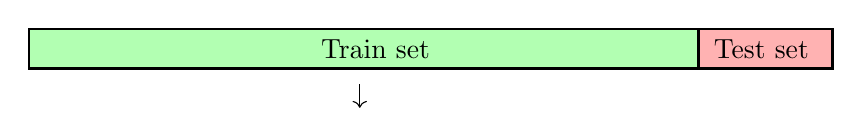
\begin{tikzpicture}
		\draw[line width=1pt, fill=green!30] (0,0) rectangle (8.5cm,0.5cm);
		\draw[line width=1pt, fill=red!30] (8.5cm,0) rectangle (10.2cm,0.5cm);
    \node at (4.4cm, 0.25cm) {Train set}; 
    \node at (9.3cm, 0.25cm) {Test set};  
		\draw[->] (4.2cm,-0.2cm) -- (4.2cm,-0.5cm);
\end{tikzpicture}

				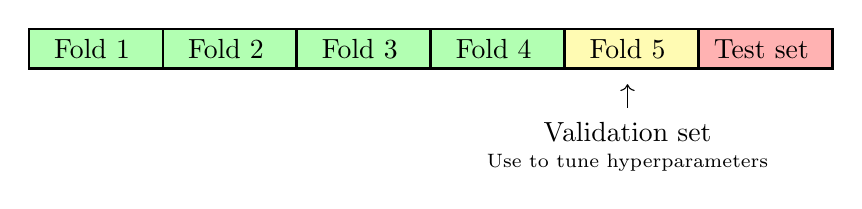
\begin{tikzpicture}
    \draw[line width=1pt, fill=green!30] (0,0) rectangle (10.2cm,0.5cm); 
		\draw[line width=1pt, fill=green!30] (1.7cm,0) rectangle (3.4cm,0.5cm);
		\draw[line width=1pt, fill=green!30] (3.4cm,0) rectangle (5.1cm,0.5cm);
		\draw[line width=1pt, fill=green!30] (5.1cm,0) rectangle (6.8cm,0.5cm);
		\draw[line width=1pt, fill=yellow!30] (6.8cm,0) rectangle (8.5cm,0.5cm);
		\draw[line width=1pt, fill=red!30] (8.5cm,0) rectangle (10.2cm,0.5cm);
		\node at (0.8cm, 0.25cm) {Fold 1}; 
		\node at (2.5cm, 0.25cm) {Fold 2}; 
		\node at (4.2cm, 0.25cm) {Fold 3}; 
		\node at (5.9cm, 0.25cm) {Fold 4}; 
		\node at (7.6cm, 0.25cm) {Fold 5}; 
		\node at (9.3cm, 0.25cm) {Test set}; 
		\draw[<-] (7.6cm,-0.2cm) -- (7.6cm,-0.5cm);
		\node at (7.6cm, -0.8cm) {Validation set};  
		\node[font=\scriptsize] at (7.6cm, -1.2cm) {Use to tune hyperparameters};  
\end{tikzpicture}

	\begin{itemize}
		\item Loop through all folds to be the validation fold
		\item Other folds build the train set
		\item Average performance values
	\end{itemize}
    \end{frame}
		\begin{frame}{What do we mean by learning? - revised} \pause
		Learning: Based on training data, finding a model with parameters $\boldsymbol{w}$ that generalizes well.  \pause
		
		In machine learning models are often called \emph{estimators} or \emph{hypotheses}.
		%\begin{itemize}
		%\item Empirical risk minimization view:
			%\begin{itemize}
				%\item Predictor as a function
				%\item Loss function
				%\item Regularization \pause
			%\end{itemize}
			%\item Probabilistic view:
			%\begin{itemize}
				%\item Predictor (estimator) as a probabilistic model
				%\item Likelihood
				%\item Prior
				%\item[$\rightarrow$] Estimating parameters based on data
			%\end{itemize}
	%\end{itemize}
    \end{frame}
		
		\section{Properties of Estimators}
		\begin{frame}{Properties of estimators}
		%
		\begin{itemize}
				\item Good estimator: Function whose output is close to the true underlying function that generated the training data. \pause
				\item How can we tell, if an estimator is any good?
				\item[$\rightarrow$] We can analyze two most common properties of estimators:
				\begin{itemize}
					\item Bias
					\item Variance
				\end{itemize}
			\end{itemize}
    \end{frame}
			\begin{frame}{Bias}
		\begin{itemize}
				\item What is the inherent error that persists in your estimator, even when trained with an unlimited amount of data?
				\item The error that arises because the estimator leans towards a particular type of solution (e.g. linear regression)
				\item Bias is an inherent characteristic of the model
			\end{itemize}
    \end{frame}
		\begin{frame}{Variance}
		\begin{itemize}
				\item Measures, how much we expect the estimator to vary as a function of the data sample, i.e. if we were to independently re-sample the dataset from the underlying data generating process
				\item To what extent does the estimator exhibit excessive specialization to a specific training set (overfitting)?
			\end{itemize}
    \end{frame}
		{ \referencefootnote{Image was taken from \cite{Goodfellow_et_al_2016}}
		\begin{frame}{Bias-Variance tradeoff}
			\begin{figure}
					\center
					\includegraphics[scale=.45]{figures/biasvariance.png}
					\caption{The relationship between bias and variance is tightly linked to the concepts of underfitting, overfitting and model capacity.}
        \end{figure}
    \end{frame}
		\note{Imagine we take five different data sets of the same problem. We train the same model 5 times. High bias, low variance means that all 5 estimators have consistently bad predictions. High variance, low bias means that the predictions are good on average, but vary a lot. (Dartscheibe zeichnen.)}
		}
\begin{frame}{Refs}
\printbibliography
\end{frame}


\end{document}
